This section discusses the method used to perform the thermal analysis of the \gls{tps}. First the required input and output are explained, then the analysis method is briefly described. The limitations of the model and concluding remarks will conclude this section.

\paragraph{Input and output}
To perform the thermal analysis the following input is needed. A given lay-up that consists of different materials with variable thicknesses. From the aerodynamic analysis and the wall temperature ($\gls{sym:T}_w$) a heat flux ($\gls{sym:qdot}_s$) is found. The chosen trajectory, which results from the orbit analysis, determines the atmospheric temperature ($\gls{sym:T}_{atm}$). Using the given lay-up, the heat flux and atmospheric trajectory as input in the upcoming analysis method, the temperature distribution through the layup and over time is found. This distribution also consists of the wall temperature ($\gls{sym:T}_w$), which is used to determine the heat flux. Thus, herein a small iteration takes place. After the temperature distribution is obtained it is be used to check whether a given lay-up will properly function in the chosen trajectory.

\paragraph{Assumptions}
Here the assumptions are stated that are used to simplify the problem.
\begin{itemize}
	\item The aerodynamic analysis has shown that the highest heat flux is found in the stagnation point at the wall. Therefore this is the point of interest for which the whole \gls{tps} is sized.
	\item The sizing can be done in one point with a one dimensional lay-up since the one dimensional analysis is very comparable to the three dimensional analysis at the centre of the heat shield according to Del Corso et al \cite{Corso2009}.
	\item It is assumed that used materials have constant properties as the temperature changes. 
	\item The heat equation used to model the problem can be discretised. The Crank-Nicolson scheme is used as discretisation scheme, which has as advantage that it is unconditionally stable.
	\item The contact resistance between the layers can be modelled as a thin layer of air with varying thermal conductivity.
	\item The incoming heat flux only consists of the aerodynamic heating. Influences such as the solar flux, Mars' albedo and Mars' infra-red radiation are considered negligible with respect to the aerodynamic heating.
\end{itemize}


\paragraph{Analysis method}
Figure \ref{fig:1dmodelthermal} is used to model the problem. Smith et al have modelled the problem in approximately the same way and therefore used as reference for the to be developed model \cite{Smith2011}. It start with a given lay-up consisting of thermal protection, insulation and structural layers. The heat transfer is modelled by an incoming heat flux due to the convective aerodynamic heating at the surface and an outgoing radiation at the surface and back. In between the surface and the back the different layers are separated by a layer with varying conductivity that models the contact resistance. Within the layers heat is transferred by conduction.

\begin{figure}[h]
	\centering
	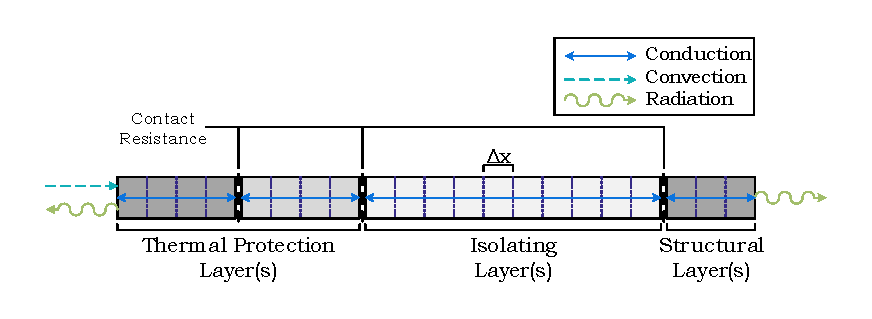
\includegraphics{./Figure/Thermal/1dmodelthermal.pdf}
	\caption{One-dimensional thermal model}
	\label{fig:1dmodelthermal}
\end{figure}

Since a one-dimensional thermal model is used to analyse the problem, Equation \eqref{eq:thermheat} or the one-dimensional heat equation can be used to relate the required temperature, space and time using the thermal diffusivity ($\gls{sym:alphat}$). The thermal diffusivity is a function of the thermal conductivity ($\gls{sym:k}$), density ($\gls{sym:rho}$) and specific heat capacity ($\gls{sym:cp}$) as shown in Equation \eqref{eq:thermdif} \cite{Holman2002}. A Crank-Nicolson scheme is used to implement the heat equation. This will model the conduction within the layers. The convective heating is obtained from the aerodynamic analysis and the radiation is calculated using Equation \eqref{eq:thermrad} \cite{Holman2002}. It is assumed that the temperature ($\gls{sym:T}_\infty$) into which the heat shield radiates is equal to the atmospheric temperature of Mars, which is obtained from the chosen trajectory.

\begin{multicols}{3}
\begin{equation}
\frac{\partial \gls{sym:T}}{\partial \gls{sym:t}} = \gls{sym:alphat}\frac{\partial^2\gls{sym:T}}{\partial \gls{sym:x}^2}
\label{eq:thermheat}
\end{equation}\break
\begin{equation}
\gls{sym:alphat} = \frac{\gls{sym:k}}{\gls{sym:rho}\gls{sym:cp}}
\label{eq:thermdif}
\end{equation}\break
\begin{equation}
\gls{sym:qdot}_r = \gls{sym:eps}\gls{con:stefanboltzmann}\left(\gls{sym:T}_w^4-\gls{sym:T}_\infty^4\right)
\label{eq:thermrad}
\end{equation}
\end{multicols}


\paragraph{Limitations}
Simplifying the problem introduces some limitations to the design tool. One of the drawbacks of a one-dimensional analysis is that the complete \gls{tps} is sized according to the conditions at the stagnation point. Furthermore it does not account for heat flowing across the other plane that is not being analysed. These drawbacks will decrease the estimated heat through the lay-up and therefore the current analysis method provides a conservative estimate for the \gls{tps}. 

The assumption that material properties do not vary with temperature is made as the influence of this is relatively small on the required thicknesses of different lay-ups. Note that this will not lead to a more conservative design as the thermal resistance decreases as temperature increases. 

The paper by Del Corso et al states that it is difficult to analytically determine the contact resistance \cite{Corso2009}. The paper used their own data for this, however arbitrary multiplication factors had to be applied to match their model with validation data. Also analytically calculating the contact resistance introduces more unknowns that have to be determined. Therefore varying conductivities have been empirically assigned to the thin layers of air between the layers. Disadvantage is that multiple layers had to be tested to find correct conductivities such that the developed tool matches experimental data. Experimental data is provided in paper by Del Corso et al \cite{Corso2009,Corso2011}. Before the actual design can be conducted, the thermal model must be verified and validated as is done in Appendix \ref{sec:VandVthermo}.



